\chapter{Distanze}
	\section{Distanza punto - piano}
		Dati un piano ed un punto nello spazio definiti come i seguenti:
		$$ \pi = ax + by + cz = d \: , \qquad P_0=(x_0, y_0, z_0) $$
		La distanza fra di essi è pari a
		$$ d(P_0, \pi) = \frac{\vert a x_0 + by_0 + cz_0 - d \vert}{\sqrt{a^2 + b^2 + c^2}} $$
		\begin{GrayBox}
			\paragraph{Dimostrazione}
			\begin{center}
				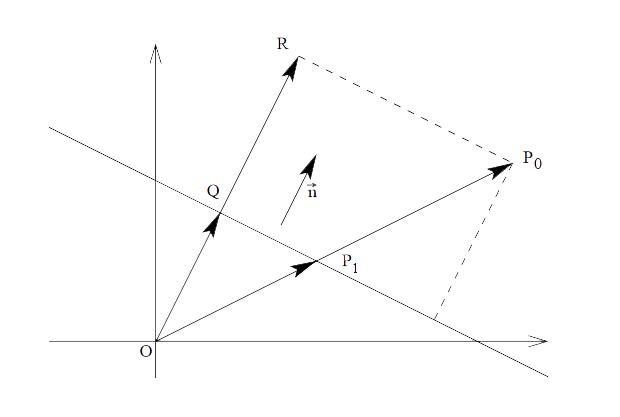
\includegraphics[width=\textwidth]{distanza-punto-piano}
			\end{center}
			La distanza fra il punto ed il piano è pari alla lunghezza del segmento $ \overrightarrow{QR} $: tale segmento non è altro che la proiezione di $ \overrightarrow{P_1P_0} $ nel versore normale \textit{n} del piano \footnote{$ \vec{n} = \frac{(a, b, c)}{\sqrt{a^2 + b^2 + c^2}} = (\frac{a}{\sqrt{a^2 + b^2 + c^2}}, \frac{b}{\sqrt{a^2 + b^2 + c^2}}, \frac{c}{\sqrt{a^2 + b^2 + c^2}})$  è il versore normale del piano (la sua lunghezza, per definizione, è pari ad uno}.
			$$ d (P_0, \pi) = \Vert \overrightarrow{QR} \Vert = \Vert pr_{\vec{n}}(\overrightarrow{P_1P_0}) \Vert $$
			Ricordando che la formula per trovare la proiezione di un vettore su un altro è $ pr_y(x) = \frac{x \cdot y}{\Vert y \Vert^2} \cdot y $, la lunghezza della proiezione di $ \overrightarrow{P_1P_0} $ è
			$$ pr_{\vec{n}}(\overrightarrow{P_1P_0}) = \frac{\overrightarrow{P_1P_0} \cdot \vec{n}}{\Vert \vec{n} \Vert^2} \cdot \vec{n} $$
			Dato che, per definizione, la lunghezza del versore $\vec{n}$ è 1, il denominatore di tale equazione viene sottinteso essere uguale ad 1.
			$$ d(P_0, \pi) = \vert \overrightarrow{P_1P_0} \cdot \vec{n} \vert $$
			Il risultato di tale prodotto vettoriale è il seguente:
			$$ \vert \overrightarrow{P_1P_0} \cdot \vec{n} \vert = \Big\vert \frac{a \cdot (x_0 - x_1) + b \cdot (y_0 - y_1) + c \cdot ( z_0 - z_1 )}{\sqrt{a^2 + b^2 + c^2}} \Big\vert $$
			Dato che $P_1$ può essere un punto qualsiasi nel piano, il prodotto fra le coordinate del piano e quelle di tale punto possono essere raggruppate nell'intercetta $d$:
			$$ d (P_0, \pi) = \frac{\vert a x_0 + b y_0 + c z_0 - d \vert}{\sqrt{a^2 + b^2 + c^2}} $$
			Nel piano la distanza fra un punto ed una retta è analoga alla precedente, viene esclusa la terza dimensione
			$$ d (P_0, r) = \frac{\vert a x_0 + b y_0 - c \vert}{\sqrt{a^2 + b^2}} \quad , \text{ con } r = ax + by = c $$
		\end{GrayBox}

	\section{Distanza punto - retta}
		Dati una retta ed un punto nello spazio, per poter trovare la distanza fra di essi è necessario ottenere il piano ortogonale alla retta e passante per il punto; la distanza fra il punto di intersezione tra il piano e la retta ed il punto iniziale sarà pari alla distanza fra quest'ultimo e la retta.
		
		\begin{GrayBox}
			\paragraph{esempio}
			Dati
			$$ P_0 = (1, 2, 1) \qquad \qquad r = \begin{cases}
				x = 2t \\
				y = t \quad , \: t \in \mathbb{R} \\
				z = t
			\end{cases} $$
		trovare la distanza fra di essi.
		
		\begin{enumerate}
			\item ricavo la normale al piano $ \pi \bot r \, : \, P_0 \in \pi $:  $ \vec{v} = (2, 1, 1) $
			\item scrivo l'equazione del piano facendo uso della normale e delle coordinate del punto P: $ \pi = 2 \cdot (x - 1) + (y - 2) + (z - 1) = 0 $
			\item sostituisco le coordinate di \textit{r} all'interno dell'equazione del piano per trovare la loro intersezione \textit{Q}:
			$$ Q : \, 2 (2t - 1) + (t - 2) + (t - 1) = 0 \implies t = 5/6 $$
			$$ \text{sostituisco... } Q = (\frac{5}{3}, \frac{5}{6}, \frac{5}{6}) $$
			\item la distanza fra $P_0$ e \textit{Q} è pari a quella fra $P_0$ ed r:
			$$ d (P_0, r) = d (P_0, Q) = \Vert \overrightarrow{P_0Q} \Vert = ... $$
		\end{enumerate}
		\end{GrayBox}
	\section{Distanza fra rette parallele nello spazio}
		\subsection{nello spazio}
			la distanza fra di esse è pari alla distanza fra i loro punti di intersezione con il piano $\pi$ a loro ortogonale.
			
		\subsection{nel piano}
			la distanza fra di esse è pari a quelli che vi è fra i loro punti di intersezione con una retta a loro parallela ($ m_s = - \frac{1}{m_r} $).
	
	\section{Distanza fra rette sghembe}
		Date le rette $r$ e $r'$, vi sono due metodi per trovare la distanza fra di esse.
		
		\subsection{I metodo}
			Definiamo i punti $P \in r$ e $Q \in r'$ le cui coordinate sono pari alle coordinate parametriche delle due rette.
			
			Troviamo il vettore $\overrightarrow{PQ}$ e, dato che quest'ultimo deve essere perpendicolare alle due rette, il suo prodotto vettoriale con i vettori direttori delle rette deve essere pari a 0.
			$$ \begin{cases}
				\overrightarrow{PQ} \cdot \vec{v} = 0 \\
				\overrightarrow{PQ} \cdot \vec{v'} = 0
			\end{cases}$$
		
			Risolvendo tale sistema è possibile trovare i due parametri \textit{t} ed \textit{s}, relativi rispettivamente alle rette \textit{r} e \textit{r'}; sostituendo tali parametri nei punti \textit{P} e \textit{Q}, è possibile trovare le coordinate dei due punti la cui distanza è pari a quella fra le due rette sghembe.
		
		\subsection{II metodo}
			Definisco il fascio dei piani contenenti \textit{r'}:
			$$ \lambda \cdot (\text{eq. cartesiana 1}) + \mu \cdot (\text{eq. cartesiana 2}) = 0 $$
			Il piano che dobbiamo identificare deve essere parallelo a \textit{r}, dunque la sua normale (le cui coordinate sono pari ai coefficienti nell'equazione del fascio) deve essere perpendicolare alla direttrice di \textit{r}
			$$ \pi \parallel r \iff \vec{n} \bot \vec{v} \iff \vec{n} \cdot \vec{v} = 0 $$
			Facendo ciò è possibile trovare la relazione che lega i due parametri $\lambda$ e $\mu$, fissandone uno sarà possibile trovare anche l'altro.
			
			Una volta sostituiti i due parametri nell'equazione del fascio di piani sarà possibile ottenere il piano che cercavamo, la sua distanza da un punto $P_0 \in r$ è pari a quella fra le due rette sghembe.